\ifspanish

\question La v.a. $X$ con ddp
$$ p_X(x) =
					      \left\{\begin{array}{ll}
						  	\displaystyle
								  1, & 0<x<1 \\
	  							  0, & {\mbox{en otro caso}} 
	 					 \end{array} 
						  \right.						  $$
se transforma como indica en la figura, dando lugar a la v.a. observable $Y$.

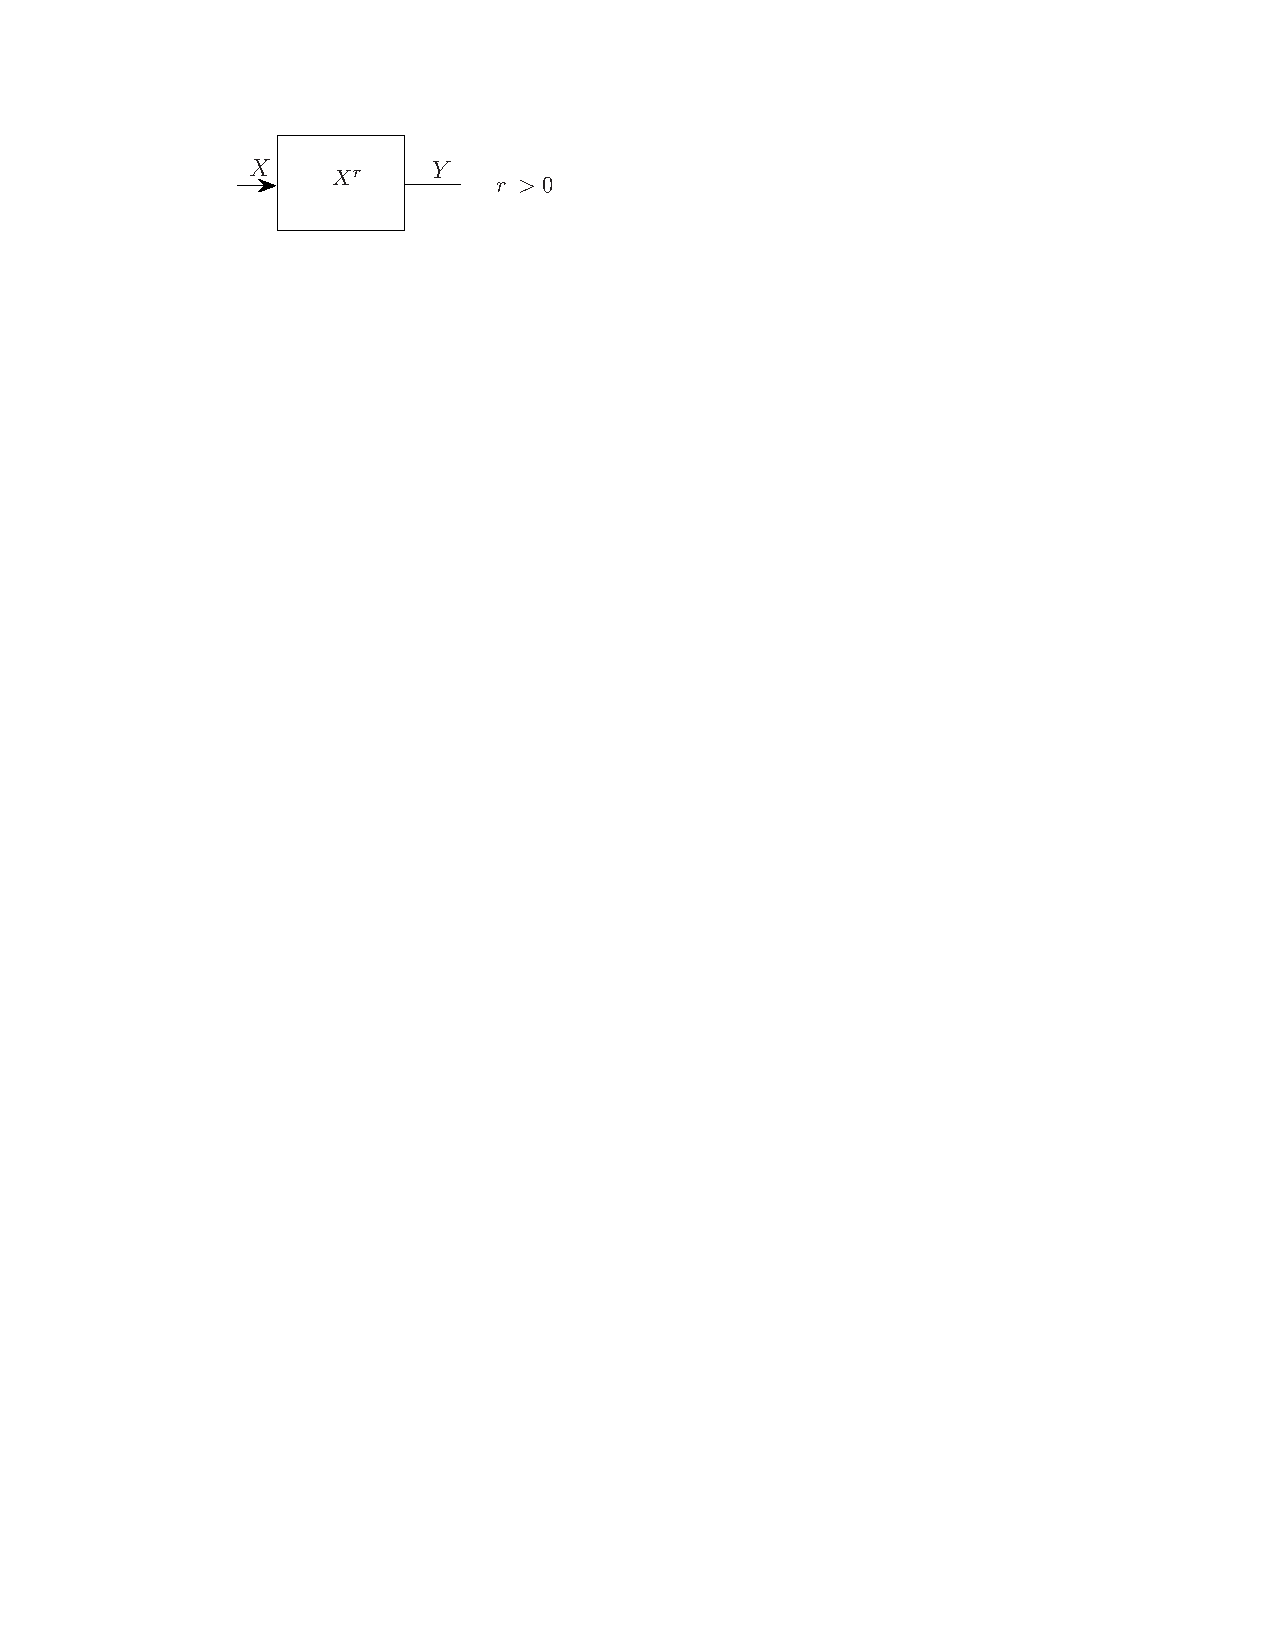
\includegraphics[width=8cm, trim=0 24cm 12cm 2cm]{Figuras/fig28_1}

\begin{parts}
	\part Obt\'{e}ngase el estimador de m\'{a}xima verosimilitud de $r$, $\hat{R}_\text{ML}$, a partir de $K$ observaciones de $Y$ tomadas de forma independiente.
	\part Consid\'{e}rese la situaci\'{o}n \\

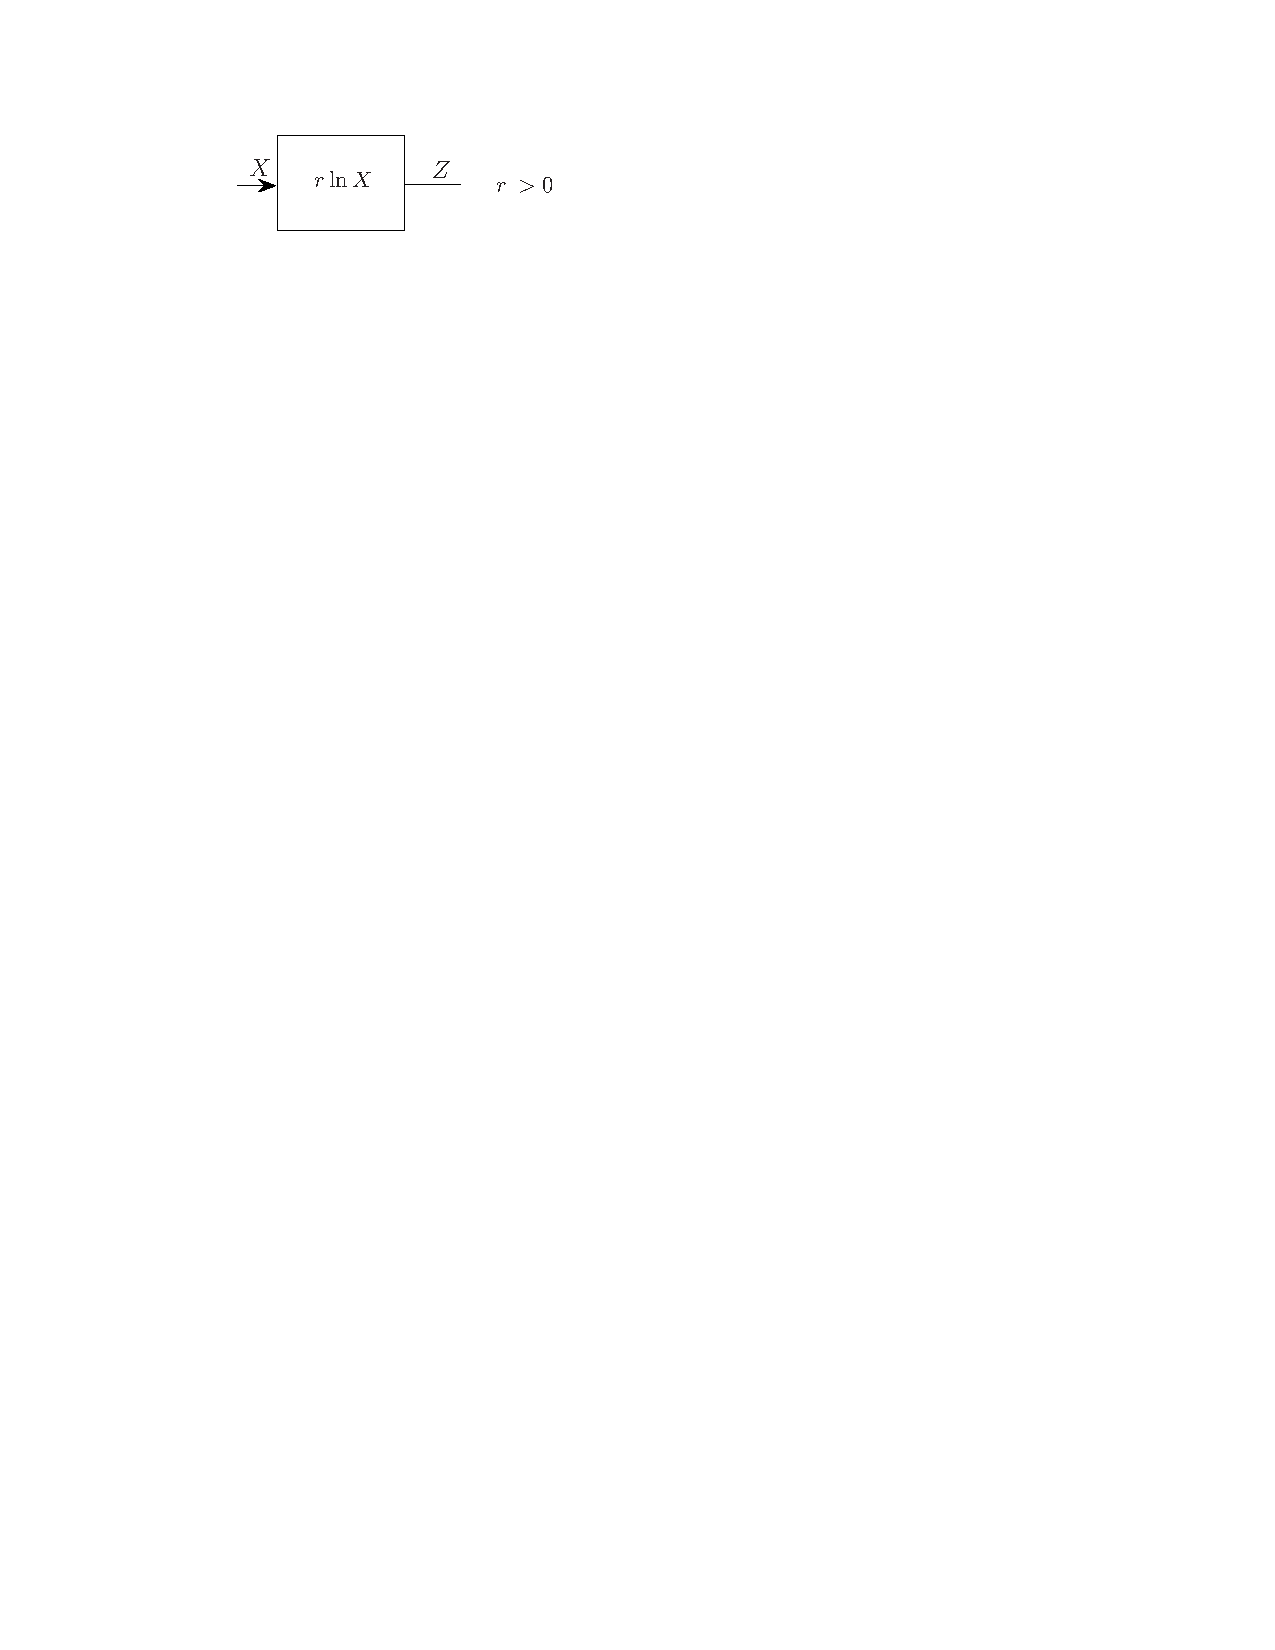
\includegraphics[width=8cm, trim=0 24cm 12cm 2cm]{Figuras/fig28_2}

y obt\'{e}ngase $\hat{R}_\text{ML}$ de $K$ observaciones de $Z$ tomadas independientemente. Com\'{e}ntese el resultado.
\end{parts}				


\begin{solution} 
  \begin{parts}
  \part $  \hat{R}_\text{ML}=-\displaystyle\frac{1}{K}\displaystyle\sum^{K}_{k=1}\ln Y^{(k)}$.  Se est\'{a} identificando el par\'{a}metro desconocido de la transformaci\'{o}n.
  \part $  \hat{R}_\text{ML}=-\displaystyle\frac{1}{K}\displaystyle\sum^{K}_{k=1} Z^{(k)}$. Coincide con el anterior: $Z=\ln Y$, ya que implica una transformaci\'{o}n invertible de $Y$. 
  \end{parts}
\end{solution}

\else

\question A random variable $X$ with p.d.f.
$$ p_X(x) =
					      \left\{\begin{array}{ll}
						  	\displaystyle
								  1, & 0<x<1 \\
	  							  0, & {\mbox{otherwise}} 
	 					 \end{array} 
						  \right.						  $$
is transformed as indicated in the figure, producing a random observation $Y$.

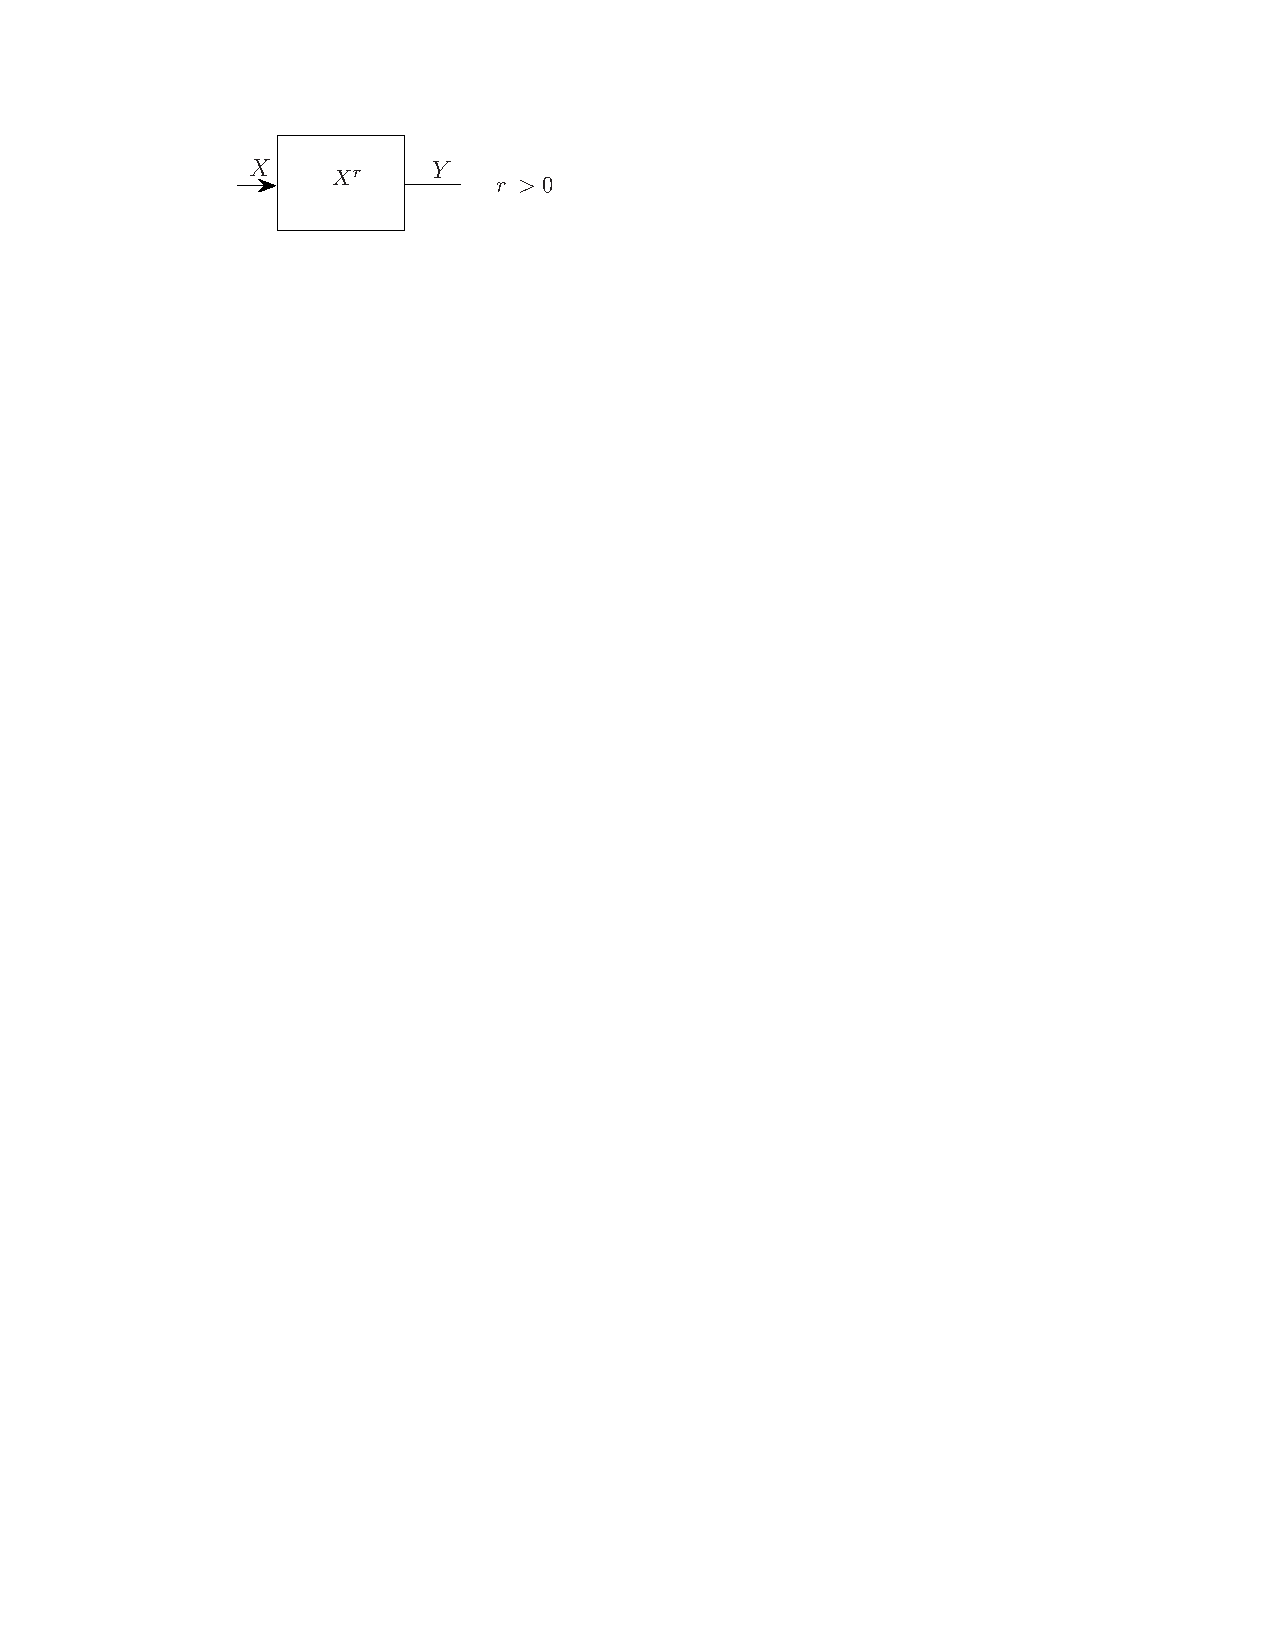
\includegraphics[width=8cm, trim=0 24cm 12cm 2cm]{Figuras/fig28_1}

\begin{parts}
	\part Obtain the maximum likelihood estimator of $r$, $\hat{R}_\text{ML}$, based on $K$  independently drawn observations of $Y$.
	\part Now, consider the following situation \\

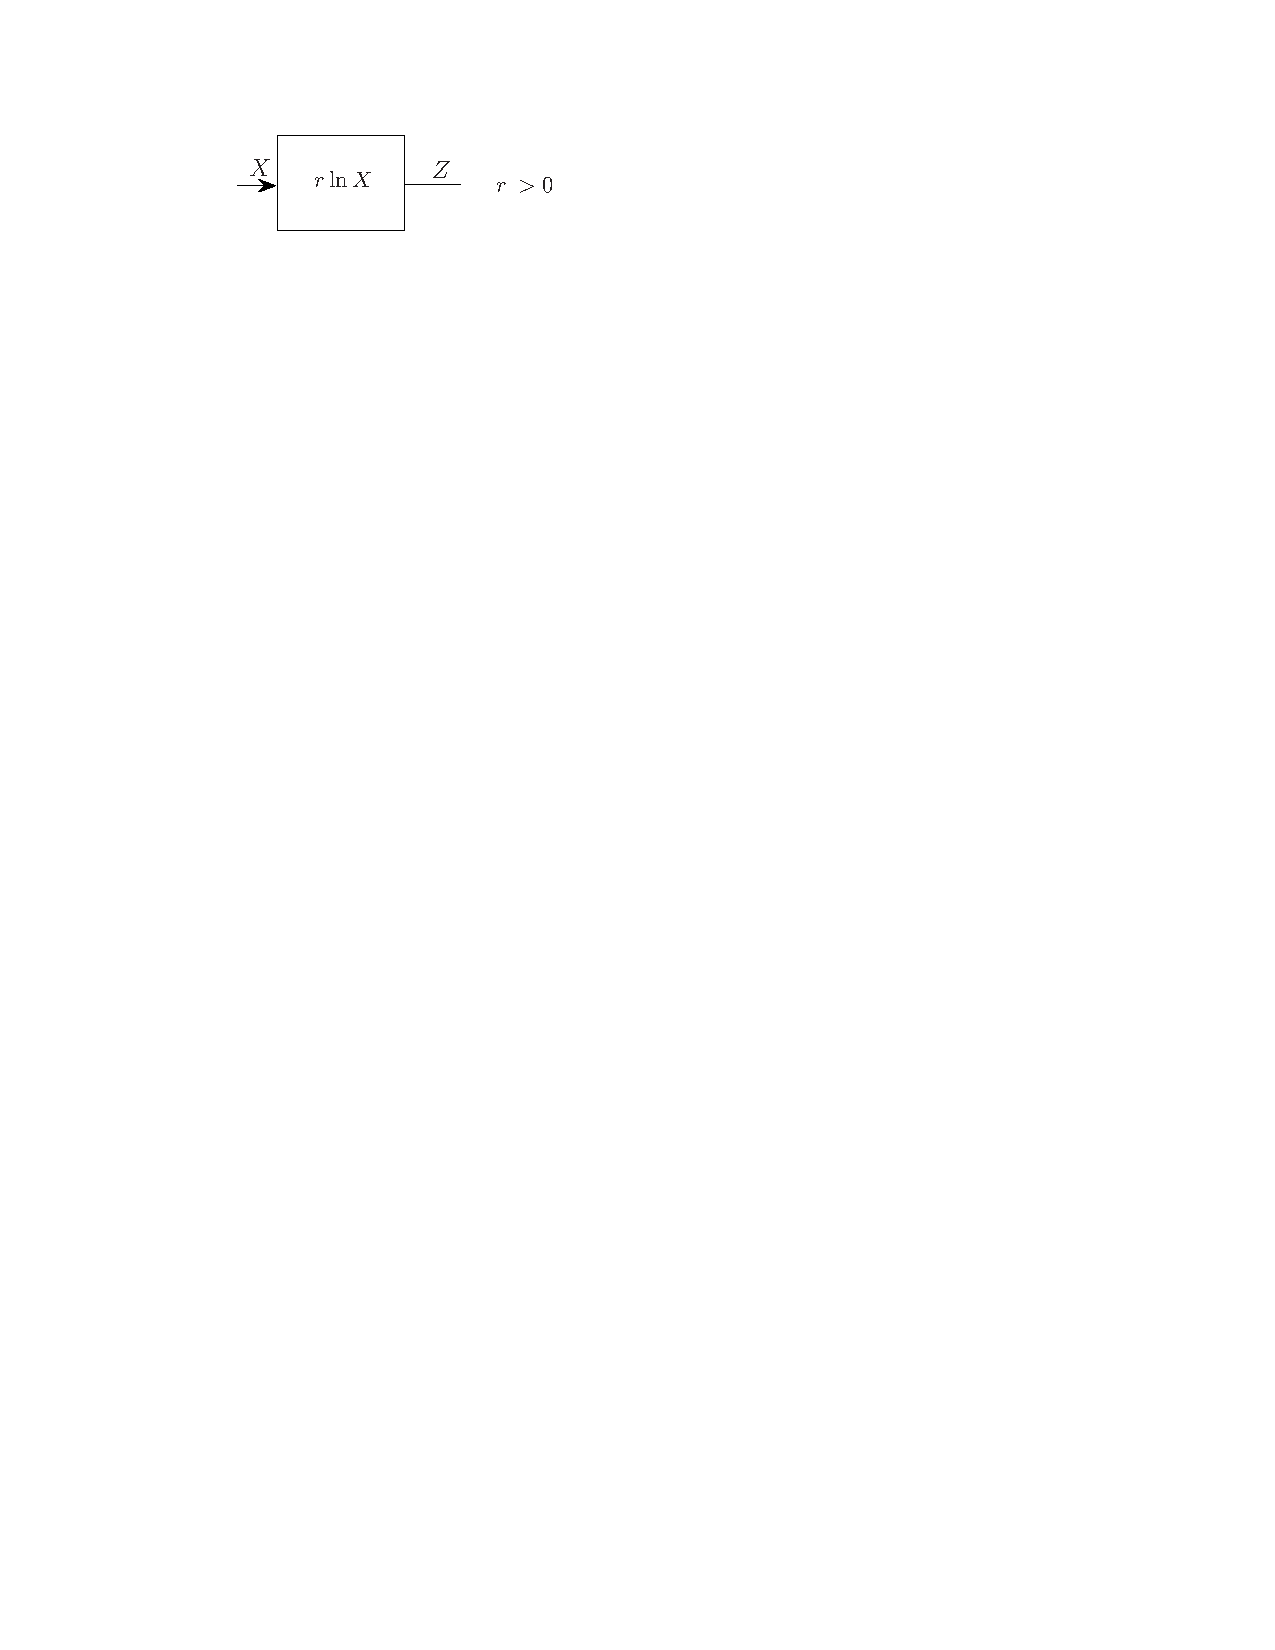
\includegraphics[width=8cm, trim=0 24cm 12cm 2cm]{Figuras/fig28_2}

and obtain $\hat{R}_\text{ML}$ using $K$ independent observations of random variable $Z$.  Discuss your result.
\end{parts}				


\begin{solution} 
  \begin{parts}
  \part $\hat{R}_\text{ML}=-\displaystyle\frac{1}{K}\displaystyle\sum^{K}_{k=1}\ln Y^{(k)}$.  The unknown parameter of the transformation is being identified.
  \part $\hat{R}_\text{ML}=-\displaystyle\frac{1}{K}\displaystyle\sum^{K}_{k=1} Z^{(k)}$. It is coherent with the previous estimator since $Z=\ln Y$, which is a deterministic (and invertible) transformation of $Y$. 
  \end{parts}
  \end{solution}

\fi